\renewcommand{\baselinestretch}{1.5}
\chapter{\texttt{ABC} visualisation}
\label{App:abc}
\begin{figure}[htbp]
    \centering
    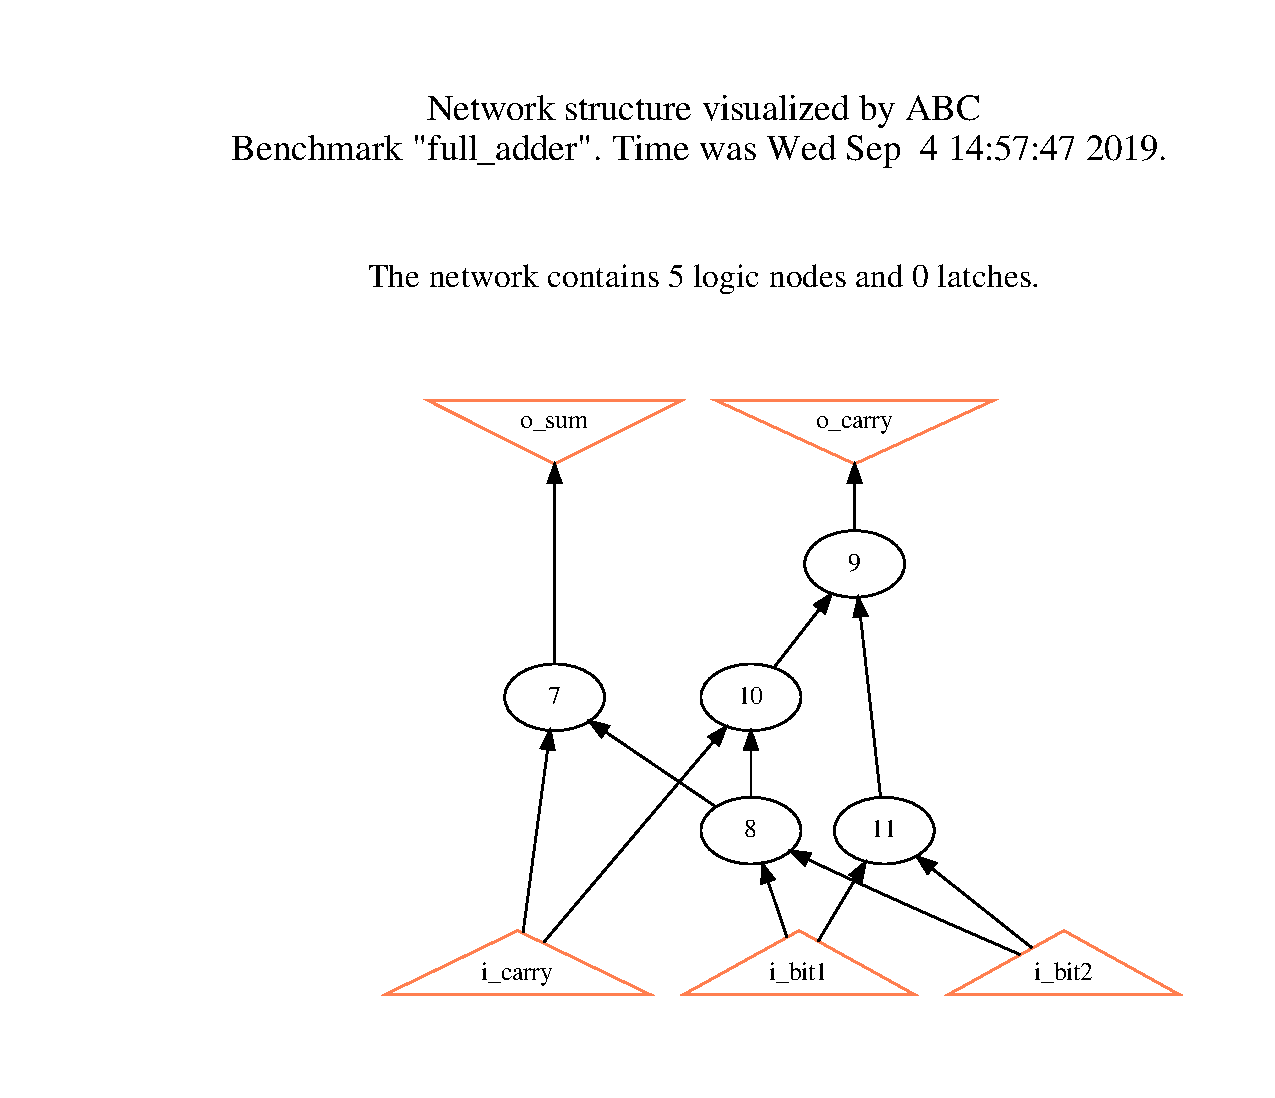
\includegraphics[width=15cm]{MScThesisTemplate/Figs/renode.pdf}
    \caption{\footnotesize renode}
\end{figure}
\begin{figure}[htbp]
    \centering
    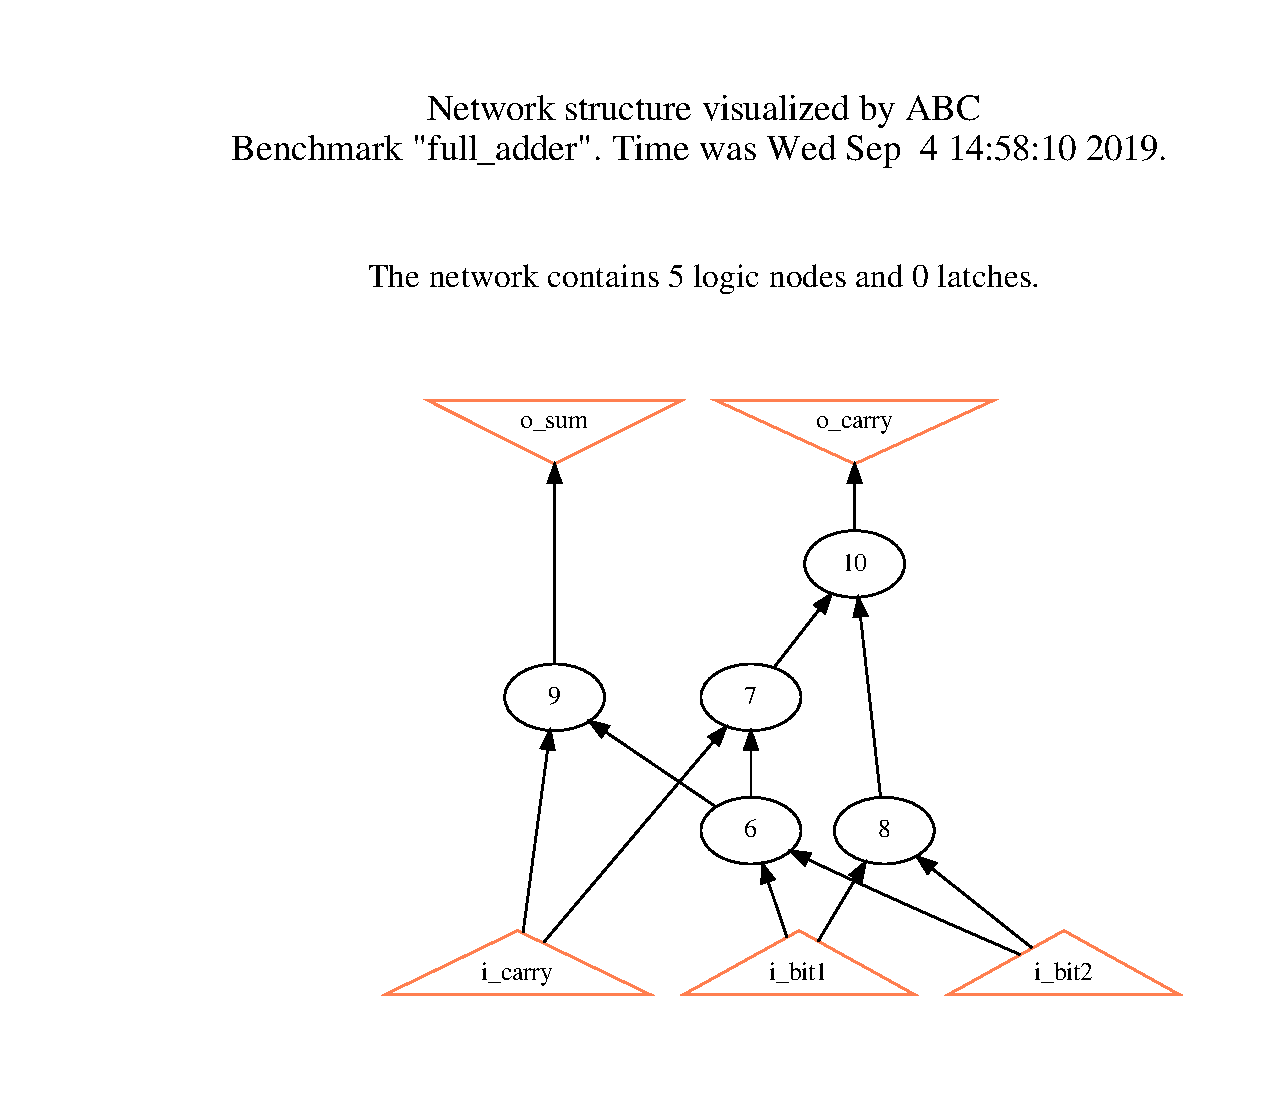
\includegraphics[width=15cm]{MScThesisTemplate/Figs/cleanup.pdf}
    \caption{\footnotesize cleanup}
\end{figure}
\begin{figure}[htbp]
    \centering
    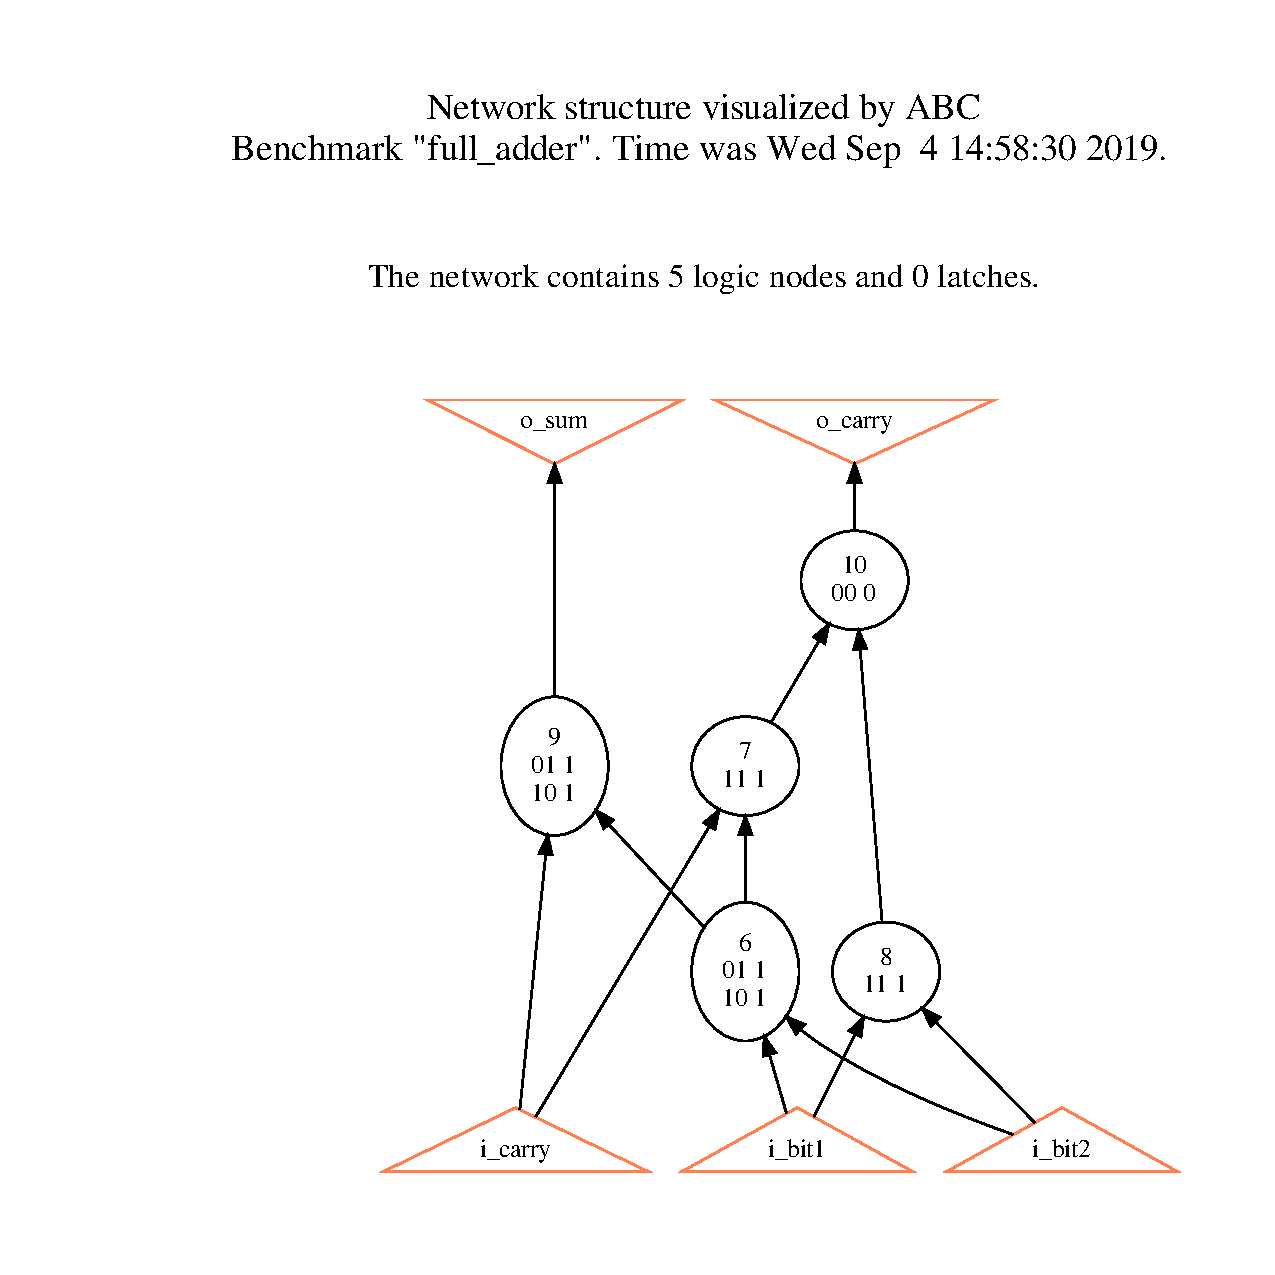
\includegraphics[width=15cm]{MScThesisTemplate/Figs/sweep.pdf}
    \caption{\footnotesize sweep}
\end{figure}
\begin{figure}[htbp]
    \centering
    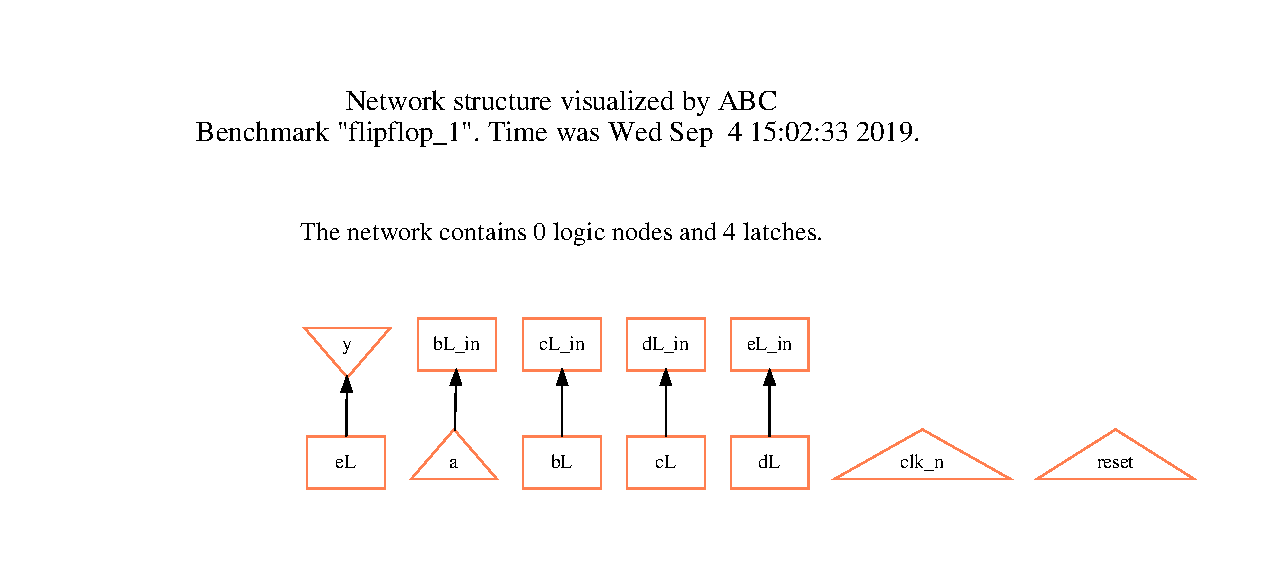
\includegraphics[width=15cm]{MScThesisTemplate/Figs/cycle.pdf}
    \caption{\footnotesize cycle}
\end{figure}
\begin{figure}[htbp]
    \centering
    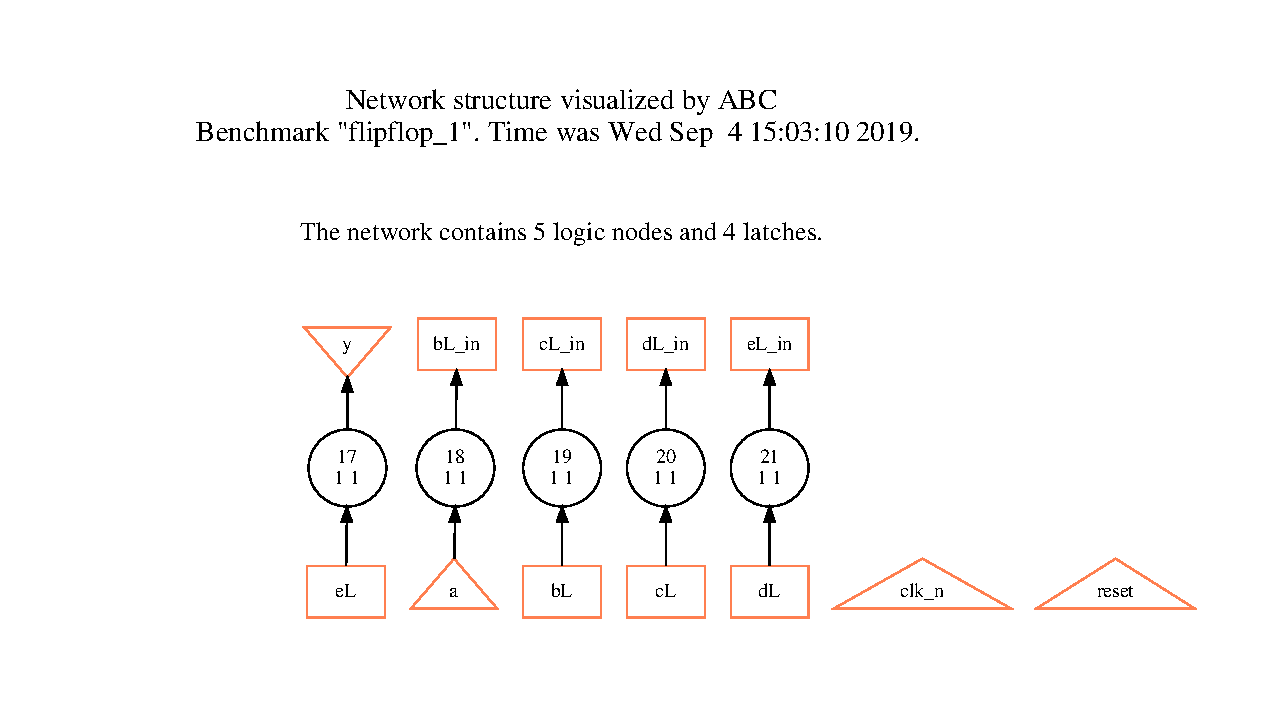
\includegraphics[width=15cm]{MScThesisTemplate/Figs/retime.pdf}
    \caption{\footnotesize retime}
\end{figure}
\begin{figure}[htbp]
    \centering
    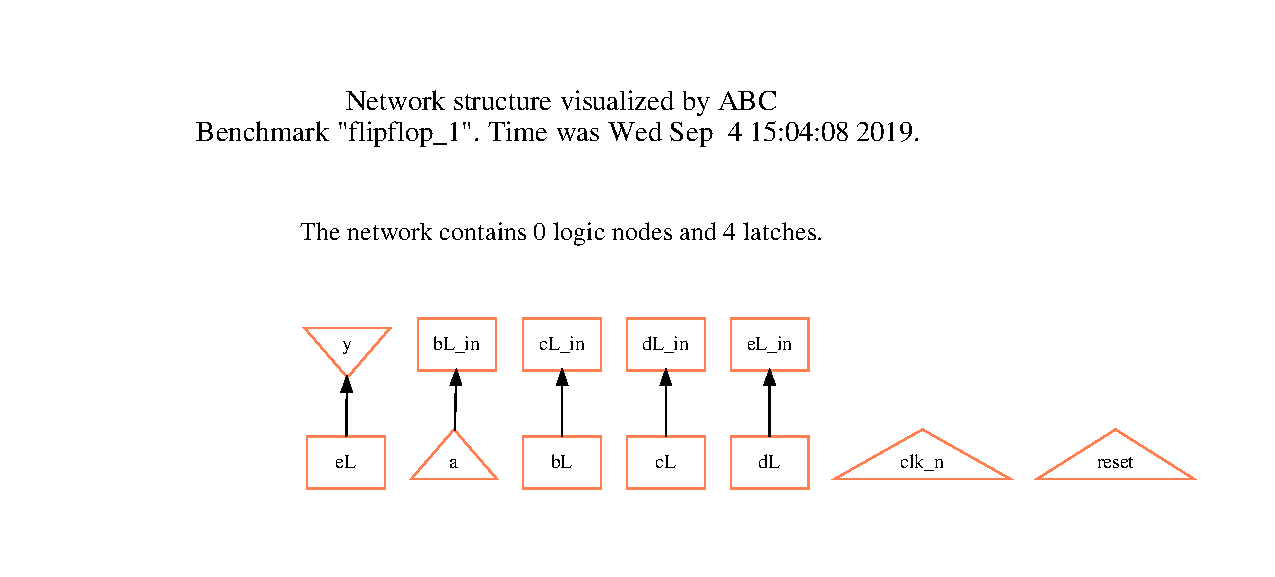
\includegraphics[width=15cm]{MScThesisTemplate/Figs/scleanup.pdf}
    \caption{\footnotesize scleanup}
\end{figure}
\begin{figure}[htbp]
    \centering
    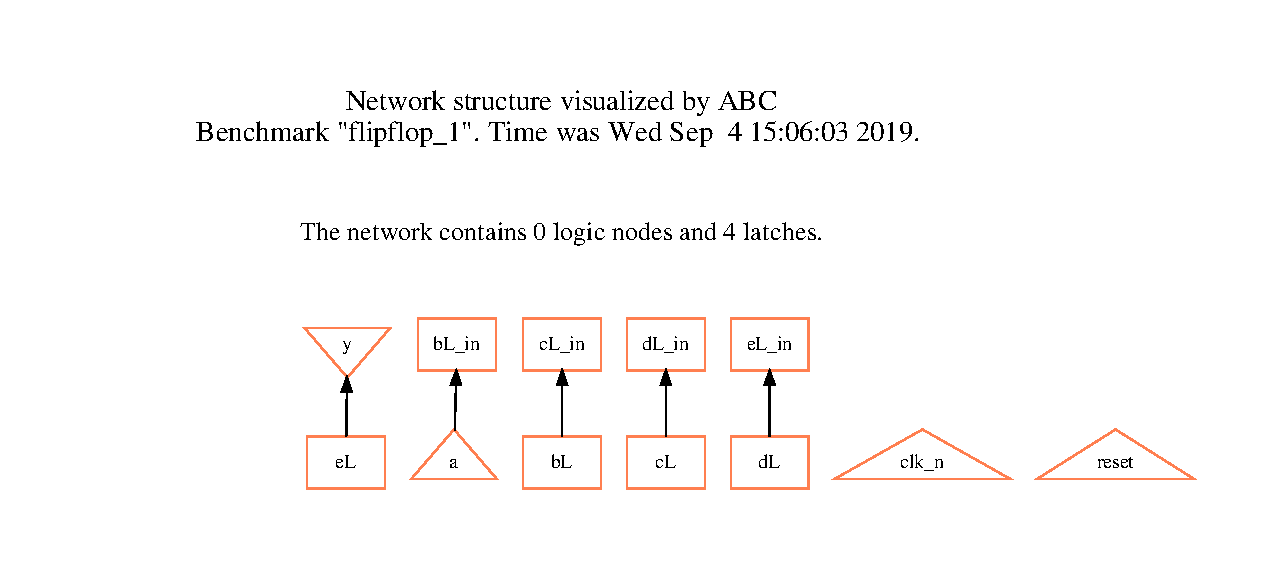
\includegraphics[width=15cm]{MScThesisTemplate/Figs/xsim.pdf}
    \caption{\footnotesize xsim}
\end{figure}